\documentclass{primedoc}
\usepackage{amsmath}
\usepackage{amssymb}
\usepackage{tikz}
\usetikzlibrary{arrows.meta}
\usepackage{microtype}
\usepackage{booktabs}
\usepackage{minted}
\setminted{style=friendly,fontsize=\small}
\renewcommand{\listoflistingscaption}{List of Code Listings}
\usepackage{hyperref}  % for hyperlinks
\usepackage[a4paper,top=4.2cm,bottom=4.2cm,left=3.5cm,right=3.5cm]{geometry} % for setting page size and margins


\usepackage[framemethod=TikZ]{mdframed}
\newcounter{thm}[section]\setcounter{thm}{0}
\renewcommand{\thethm}{\arabic{section}.\arabic{thm}}
\newenvironment{thm}[2][]{%
\refstepcounter{thm}%
\ifstrempty{#1}%
{\mdfsetup{%
frametitle={%
\tikz[baseline=(current bounding box.east),outer sep=0pt]
\node[anchor=east,rectangle,fill=blue!20]
{\strut Theorem~\thethm};}}
}%
{\mdfsetup{%
frametitle={%
\tikz[baseline=(current bounding box.east),outer sep=0pt]
\node[anchor=east,rectangle,fill=cyan!20]
{\strut Theorem~\thethm:~#1};}}%
}%
\mdfsetup{innertopmargin=10pt,linecolor=blue!20,%
linewidth=2pt,topline=true,%
frametitleaboveskip=\dimexpr-\ht\strutbox\relax
}
\begin{mdframed}[]\relax%
\label{#2}}{\end{mdframed}}


% Custom macros used in this example document
\newcommand{\doclink}[2]{\href{#1}{#2}\footnote{\url{#1}}}
\newcommand{\cs}[1]{\texttt{\textbackslash #1}}

% Frontmatter data; appears on title page
\title{Google PageRank Algorithm}
\subtitle{An Application of Linear Algebra}
\author{Manish Patel}
\softwarelogo{\includegraphics[width=8cm]{img}}
\begin{document}
\maketitle
\newpage
~\vfill
\thispagestyle{empty}
\noindent \copyright\ Manish Patel\\ % Copyright notice
\noindent \textsc{The Institute of Science, Mumbai}\\ % Publisher	
\noindent \textit{primespatel@gmail.com}\\ % URL	
\noindent \textit{2021-22}
\newpage
\tableofcontents
% \listoflistings%
\newpage

\section{Introduction}
Humans, the most successful species on the planet, used to pass on their knowledge through books, music, art, and so on. This knowledge transfer continues to this day, but with the most popular, innovative, and easily accessible source that is also a reliable alternative, you guessed it, the Internet. One can conduct a search. What exactly are prime numbers? Google returns n related pages, with the most relevant appearing first.\newline
	
\noindent The process of searching within a document collection for specific information is known as information retrieval (called a query).\\
\\
An information retrieval challenge for any document collection, especially the Web which concerns precision. The amount of accessible information continues to grow, a user's ability to look at documents does not. Users rarely look beyond the first 10 or 20 documents retrieved. This user impatience means that search engine precision must increase just as rapidly as the number of documents is increasing.\\
\\
The Web is such a unique document collection which is huge, dynamic, self-organized, and hyperlinked. The Web's self-organization means that, in contrast to traditional document collections, there is no central collection and categorization organization. The web document collection lives in a cyber warehouse, a virtual entity that is not limited by geographical constraints and can grow without limit.
\section{Elements of Web Search Engine}
	
\subsection{Crawler Module}
Web is huge and dynamic in nature as a result, all web search engines have a crawler module. This module contains the software that collects and categorizes the web's documents. The crawling software creates virtual robots, called spiders, that constantly crawls the Web gathering new information and webpages and returning to store them in a central repository.
	
\subsection{Page Repository}
The spiders return with new webpages, which are temporarily stored as complete webpages in the page repository. The new pages remain in the repository until they are sent to the indexing module, where their vital information is stripped to create a compressed version of the page.

\begin{figure}[h]
    \centering\includegraphics[scale=0.5]{engine.png}
    \caption{Elements of Web Search Engine}
    \label{fig:placeholder} % Unique label used for referencing the figure in-text
            %\addcontentsline{toc}{figure}{Figure \ref{fig:placeholder}} % Uncomment to add the figure to the table of contents
    \end{figure}

\subsection{Indexing Module}
The indexing module takes each new uncompressed page and extracts only the vital descriptors, creating a compressed description of the page that is stored in various indexes. The indexing module is like a black box function that takes the uncompressed page as input and outputs a “Cliffnotes” version of the page. The uncompressed page is then tossed out. We will be concentrating in PageRank index in this module.

\subsection{Indexes}
The indexes hold the valuable compressed information for each webpage. The first is called the content index. Here the content, such as keyword, title, and anchor text for each webpage, is stored in a compressed form using an inverted file structure. The crawler module sometimes accesses the structure index to find uncrawled pages. information regarding the hyperlink structure of pages in the search engine's index is gleaned during the indexing phase. This link information is stored in compressed form in the structure index. Special-purpose indexes are the final type of index. For example, indexes such as the image index and pdf index hold information that is useful for particular query tasks.\\
\\
The four modules above (crawler, page repository, indexers, indexes) and their corresponding data files exist and operate independent of users and their queries. Spiders are constantly crawling the Web, bringing back new and updated pages to be indexed and stored. These modules are circled and labeled as query-independent. Unlike the preceding modules, the query module is query-dependent and is initiated when a user enters a query, to which the search engine must respond in real-time.

\subsection{Query Module}
The query module converts a user's natural language query into a language that the search system can understand (usually numbers), and consults the various indexes in order to answer the query. For example, the query module consults the content index and its inverted file to find which pages use the query terms. These pages are called the relevant pages. Then the query module passes the set of relevant pages to the ranking module.

\subsection{Ranking Module}
The ranking module takes the set of relevant pages and ranks them according to some criterion. The outcome is an ordered list of webpages such that the pages near the top of the list are most likely to be what the user desires. The ranking module is perhaps the most important component of the search process because the output of the query module often results in too many relevant pages that the user must sort through. The set of relevant pages resulting from the query module is then presented to the user in order of their overall scores.
\section{PageRank Algorithm}
We are interested in calculating PageRank before calculating it, we need to know about the topology of the web.\\
\\
In order to do that, we need to view the Web as a graph. The Web's hyperlink structure forms a massive directed graph. The nodes in the graph represent webpages and the directed arcs or links represent the hyperlinks. Thus, hyperlinks into a page, which are called inlinks, point into nodes, while outlinks point out from nodes. Nodes with no outlinks are known as dangling node. We will see how it causes the PageRank.\\
	
\begin{center}
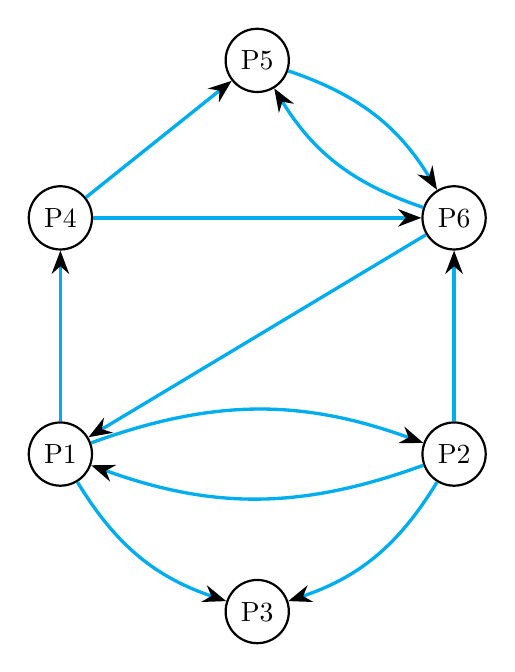
\begin{tikzpicture}
\begin{scope}[every node/.style={circle,thick,draw}]
	\node (P1) at (0,3) {P1};
	\node (P3) at (2.5,1) {P3};
	\node (P2) at (5,3) {P2} ;
	\node (P4) at (0,6) {P4};
	\node (P5) at (2.5,8) {P5};
	\node (P6) at (5,6) {P6} ;
\end{scope}			
\begin{scope}[>={Stealth[black]},
every node/.style={fill=white,circle},
every edge/.style={draw=cyan,very thick}]
\path [->] (P1) edge[bend left=20] (P2);
\path [->] (P1) edge[bend left=-20] (P3);
\path [->] (P1) edge[bend left=0] (P4);
\path [->] (P2) edge[bend left=20] (P1);
\path [->] (P2) edge[bend left=20] (P3);
\path [->] (P2) edge[bend left=0] (P6);
\path [->] (P4) edge[bend left=0] (P6);
\path [->] (P4) edge[bend left=0] (P5);
\path [->] (P5) edge[bend left=20] (P6);
\path [->] (P6) edge[bend left=0] (P1);
\path [->] (P6) edge[bend left=20] (P5);
\end{scope}
\end{tikzpicture}
\end{center}

A page is important if it is pointed to by other important pages.

\noindent Let's define PageRank of a page $P_{i}$, denoted $r\left(P_{i}\right)$ and it is the sum of the PageRanks of all pages pointing into $P_{i}$.
	
$$
r\left(P_{i}\right)=\sum_{P_{j} \in B_{P_{i}}} r\left(P_{j}\right)
$$
$B_{P_{i}}:$ is the set of pages pointing into $P_{i}$ \\
\\
The problem with formula is that the $r(P_{j})$ values, the PageRanks of pages inlinking to page $P_{i}$, are unknown. To sidestep this problem, we are going to use an iterative approach(process). That is, we are assuming that, in the beginning, all pages have equal PageRank (say, $1/n$, here $n$ is the number of web pages). As we are applying the rule in formula successively, we need to introduce some more notation in order to distinguish steps. Let $r_{k}\left(P_{i}\right)$ be the PageRank of page $P_{i}$ at $k^{th}$iteration. Then, PageRank of $P_i$ at $(k+1)^th$ iteration is given by
	
$$
r_{k+1}\left(P_{i}\right)=\sum_{P_{j} \in B_{P_{i}}} r_{k}\left(P_{j}\right)
$$
\begin{center}
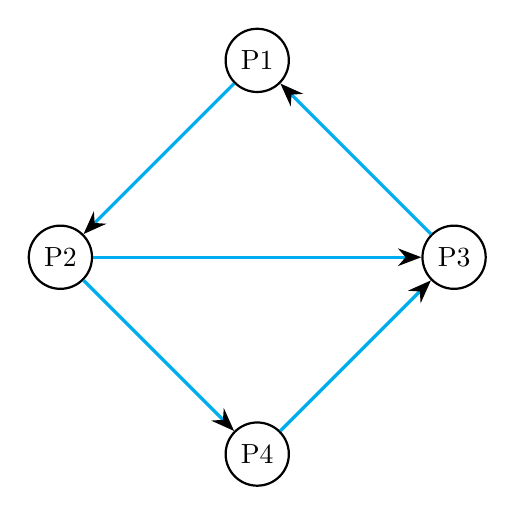
\begin{tikzpicture}
\begin{scope}[every node/.style={circle,thick,draw}]
\node (P4) at (2.5,3) {P4};
\node (P2) at (0,5.5) {P2};
\node (P1) at (2.5,8) {P1};
\node (P3) at (5,5.5) {P3} ;
\end{scope}
			
\begin{scope}[>={Stealth[black]},
every node/.style={fill=white,circle},
every edge/.style={draw=cyan,very thick}]
\path [->] (P1) edge[bend left=0] (P2);
				\path [->] (P2) edge[bend left=0] (P4);
				\path [->] (P2) edge[bend left=0] (P3);
				\path [->] (P4) edge[bend left=0] (P3);
				\path [->] (P3) edge[bend left=0] (P1);
			\end{scope}
		\end{tikzpicture}
	\end{center}
	
\noindent This process is initiated with $r_{0}\left(P_{i}\right)=1 / n$ for all pages $P_{i}$ and repeated with the hope that the PageRank scores will eventually converge to some final stable values. Applying equation to the above tiny web of 4-nodes gives the following values for the PageRanks after a few iterations.
\\

\begin{table}[h]
	\centering
	\begin{tabular}{l l l c}
		\toprule
		\textbf{Iteration 0} & \textbf{Iteration 1} & \textbf{Iteration 2} & \textbf{Iteration 3}\\
		\midrule
		$r_{0}\left(P_{1}\right)=1 / 4$ & $r_{1}\left(P_{1}\right)=1 / 4$ & $r_{2}\left(P_{1}\right)=2 / 4$ & 
		$r_{3}\left(P_{1}\right)=2 / 4$\\
		$r_{0}\left(P_{2}\right)=1 / 4$ & $r_{1}\left(P_{2}\right)=1 / 4$ & $r_{2}\left(P_{2}\right)=1 / 4$ & 
		$r_{3}\left(P_{2}\right)=2 / 4$\\
		$r_{0}\left(P_{3}\right)=1 / 4$ & $r_{1}\left(P_{3}\right)=2 / 4$ & $r_{2}\left(P_{3}\right)=2 / 4$ & 
		$r_{3}\left(P_{3}\right)=3 / 4$\\
		$r_{0}\left(P_{4}\right)=1 / 4$ & $r_{1}\left(P_{4}\right)=1 / 4$ & $r_{2}\left(P_{4}\right)=1 / 4$& 
		$r_{3}\left(P_{4}\right)=1 / 4$\\
		\bottomrule
	\end{tabular}
\end{table}

\noindent From the above table we can say that Page $P_3$ has highest rank and Page $P_4$ has lowest rank.\\
\\
\noindent This algorithm can be exploited by SEO's (Search Engine Optimization) by just creating dummy websites and pointing(more formally by giving backlinks) to their clients.\\
\\
\noindent This problem can be overcome by little change in previous algorithm.

$$
r\left(P_{i}\right)=\sum_{P_{j} \in B_{P_{i}}} \frac{r\left(P_{j}\right)}{\left|P_{j}\right|}
$$
$B_{P_{i}}:$ is the set of pages pointing into $P_{i}$ \\
$|P_{j}|:$ is the number of outlinks from page $P_{j}$.\\
\\
Recursive formula:
$$
r_{k+1}\left(P_{i}\right)=\sum_{P_{j} \in B_{P_{i}}} \frac{r_{k}\left(P_{j}\right)}{\left|P_{j}\right|} .
$$

\noindent Now, unlike previous algorithm dummy websites have no use as their value of backlinks decreases as the number of backlinks increase.

\begin{center}
	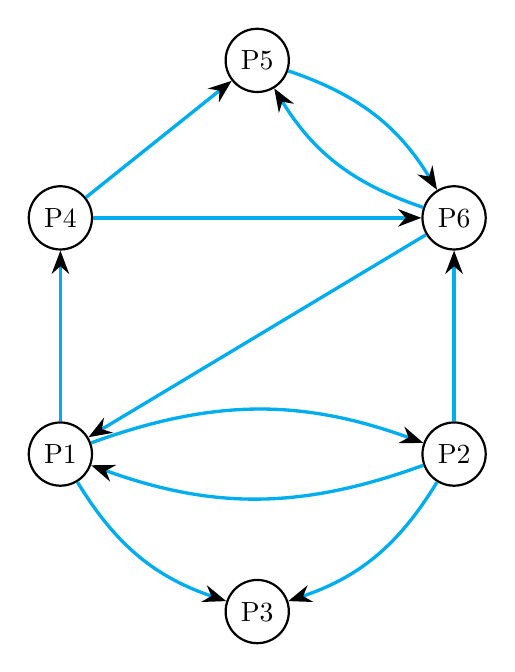
\begin{tikzpicture}
		\begin{scope}[every node/.style={circle,thick,draw}]
			\node (P1) at (0,3) {P1};
			\node (P3) at (2.5,1) {P3};
			\node (P2) at (5,3) {P2} ;
			\node (P4) at (0,6) {P4};
			\node (P5) at (2.5,8) {P5};
			\node (P6) at (5,6) {P6} ;
		\end{scope}
		\begin{scope}[>={Stealth[black]},
			every node/.style={fill=white,circle},
			every edge/.style={draw=cyan,very thick}]
			\path [->] (P1) edge[bend left=20] (P2);
			\path [->] (P1) edge[bend left=-20] (P3);
			\path [->] (P1) edge[bend left=0] (P4);
			\path [->] (P2) edge[bend left=20] (P1);
			\path [->] (P2) edge[bend left=20] (P3);
			\path [->] (P2) edge[bend left=0] (P6);
			\path [->] (P4) edge[bend left=0] (P6);
			\path [->] (P4) edge[bend left=0] (P5);
			\path [->] (P5) edge[bend left=20] (P6);
			\path [->] (P6) edge[bend left=0] (P1);
			\path [->] (P6) edge[bend left=20] (P5);
		\end{scope}
	\end{tikzpicture}
\end{center}
	
Let's calculate PageRank using updated algorithm,
	
\begin{table}[h]
	\centering
	\begin{tabular}{l l l c}
		\toprule
	\textbf{Iteration 0} & \textbf{Iteration 1} & \textbf{Iteration 2} & \textbf{PageRank}\\
		\midrule
		$r_{0}\left(P_{1}\right)=1 / 6$ & $r_{1}\left(P_{1}\right)=5 / 36$ & $r_{2}\left(P_{1}\right)=37 / 216$ & 3 \\
		$r_{0}\left(P_{2}\right)=1 / 6$ & $r_{1}\left(P_{2}\right)=2 / 36$ & $r_{2}\left(P_{2}\right)=10 / 216$ & 5 \\
		$r_{0}\left(P_{3}\right)=1 / 6$ & $r_{1}\left(P_{3}\right)=4 / 36$ & $r_{2}\left(P_{3}\right)=14 / 216$ & 4 \\
		$r_{0}\left(P_{4}\right)=1 / 6$ & $r_{1}\left(P_{4}\right)=2 / 36$ & $r_{2}\left(P_{4}\right)=10 / 216$ & 5 \\
		$r_{0}\left(P_{5}\right)=1 / 6$ & $r_{1}\left(P_{5}\right)=6 / 36$ & $r_{2}\left(P_{5}\right)=39 / 216$ & 2 \\
		$r_{0}\left(P_{6}\right)=1 / 6$ & $r_{1}\left(P_{6}\right)=11 / 36$ & $r_{2}\left(P_{6}\right)=46 / 216$ & 1\\			\bottomrule
		\end{tabular}
\end{table}
\section{Matrix Representation}

Equation compute PageRank one page at a time. Using matrices, we replace the tedious $\sum$ symbol, and at each iteration, compute a PageRank vector, which uses a single $1 \times n$ vector to hold the PageRank values for all pages in the index. In order to do this, we introduce an $n \times n$ matrix $\mathbf{H}$ and a $1 \times n$ row vector ${\pi}^{T}\geq0$ (probability vector i.e. all entries are non-negative real number with sum equal to 1). The matrix $\mathbf{H}$ is a row normalized hyperlink matrix with $\mathbf{H}_{i j}=1 /\left|P_{i}\right|$ if there is a link from node $i$ to node $j$, and 0 otherwise.
	
\begin{center}
	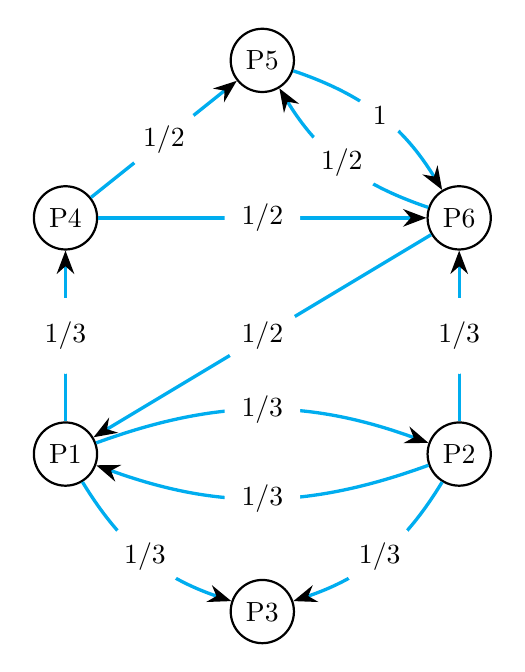
\begin{tikzpicture}
		\begin{scope}[every node/.style={circle,thick,draw}]
			\node (P1) at (0,3) {P1};
			\node (P3) at (2.5,1) {P3};
			\node (P2) at (5,3) {P2} ;
			\node (P4) at (0,6) {P4};
			\node (P5) at (2.5,8) {P5};
			\node (P6) at (5,6) {P6} ;
		\end{scope}
	\begin{scope}[>={Stealth[black]},
			every node/.style={fill=white,circle},
			every edge/.style={draw=cyan,very thick}]
			\path [->] (P1) edge[bend left=20] node {$1/3$} (P2);
			\path [->] (P1) edge[bend left=-20] node {$1/3$} (P3);
			\path [->] (P1) edge[bend left=0] node {$1/3$}(P4);
			\path [->] (P2) edge[bend left=20] node {$1/3$} (P1);
			\path [->] (P2) edge[bend left=20] node {$1/3$} (P3);
			\path [->] (P2) edge[bend left=0] node {$1/3$} (P6);				\path [->] (P4) edge[bend left=0] node {$1/2$} (P6);
			\path [->] (P4) edge[bend left=0] node {$1/2$} (P5);
			\path [->] (P5) edge[bend left=20] node {$1$} (P6);
			\path [->] (P6) edge[bend left=0] node {$1/2$} (P1);
			\path [->] (P6) edge[bend left=20] node {$1/2$} (P5);
		\end{scope}
	\end{tikzpicture}
\end{center}
	
\noindent Transition Matrix:

$$
\begin{array}{ccccccc} 
	& P_{1} & P_{2} & P_{3} & P_{4} & P_{5} & P_{6} \\
	P_{1} & 0 & 1 / 3 & 1 / 3 & 1 / 3 & 0 & 0 \\
	P_{2} & 1 / 3 & 0 & 1 / 3 & 0 & 0 & 1 / 3 \\
	P_{3} & 0 & 0 & 0 & 0 & 0 & 0 \\
	P_{4} & 0 & 0 & 0 & 0 & 1 / 2 & 1 / 2 \\
	P_{5} & 0 & 0 & 0 & 0 & 0 & 1 \\
	P_{6} & 1 / 2 & 0 & 0 & 0 & 1 / 2 & 0
\end{array}
$$

\noindent Consider last 6-node tiny web again. The $\mathbf{H}$ matrix for this graph is

$$
\mathbf{H}=\left[\begin{array}{cccccc}
	0 & 1 / 3 & 1 / 3 & 1 / 3 & 0 & 0 \\
	1 / 3 & 0 & 1 / 3 & 0 & 0 & 1 / 3 \\
	0 & 0 & 0 & 0 & 0 & 0 \\
	0 & 0 & 0 & 0 & 1 / 2 & 1 / 2 \\
	0 & 0 & 0 & 0 & 0 & 1 \\
	1 / 2 & 0 & 0 & 0 & 1 / 2 & 0
\end{array}\right]
$$

$${\pi}^{(k+1) T}={\pi}^{(k) T} \mathbf{H}$$

\noindent H is a very sparse matrix (a large proportion of its elements are 0) because most webpages link to few of other pages. ${\pi}^{(0)T}$ will be row probability vector with all entries $1/n$.

\begin{thm}[Stochastic matrix]{thm:stochasticmatrix}
A $n\times n$ Matrix A is said to be row(right) stochastic matrix if
$$
A=\left[\begin{array}{cccccc}
	a_{1,1} & a_{1,2} & \ldots & a_{1, j} & \ldots & a_{1, n} \\
	a_{2,1} & a_{2,2} & \ldots & a_{2, j} & \ldots & a_{2, n} \\
	\vdots & \vdots & \ddots & \vdots & \ddots & \vdots \\
	a_{i, 1} & a_{i, 2} & \ldots & a_{i, j} & \ldots & a_{i, n} \\
	\vdots & \vdots & \ddots & \vdots & \ddots & \vdots \\
	a_{n, 1} & a_{n, 2} & \ldots & a_{n, j} & \ldots & a_{n, n}
    \end{array}\right]
$$

$$\sum_{j=1}^{n} a_{i, j}=1$$  \centering $i = 1, 2, ..., n$
\end{thm}

\noindent H looks a lot like a stochastic transition probability matrix for a Markov chain.
The dangling nodes of the network, those nodes with no outlinks, create 0 rows in
the matrix. All the other rows, which correspond to the nondangling nodes, create
stochastic rows. Thus, We can call H as substochastic.\\

\noindent Problem with iterative process iterative equation probably caused readers, especially our mathematical readers, to ask several questions. For example,

\begin{itemize}
	\item Will this iterative process continue indefinitely or will it converge?
	\item Under what circumstances or properties of H is it guaranteed to converge?
	\item Will it converge to something that makes sense in the context of the PageRank problem?
	\item Will it converge to just one vector or multiple vectors?
	\item Does the convergence depend on the starting vector $\pi^{(0)T}$ ?
\end{itemize}
	
\subsection{Reducibility}
	
There is the problem of rank sinks, those pages that accumulate more and more PageRank at each iteration, monopolizing the scores and refusing to share. Consider the following 3-node graph,

\begin{center}
	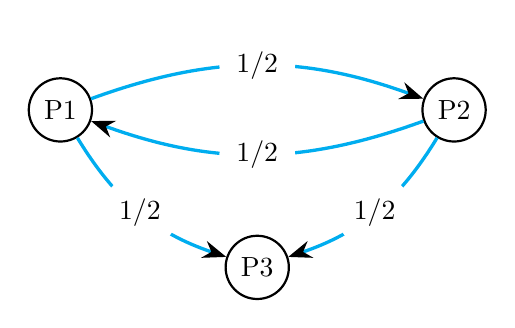
\begin{tikzpicture}
		\begin{scope}[every node/.style={circle,thick,draw}]
			\node (P1) at (0,3) {P1};
			\node (P3) at (2.5,1) {P3};
			\node (P2) at (5,3) {P2} ;
		\end{scope}
	
		\begin{scope}[>={Stealth[black]},
			every node/.style={fill=white,circle},
			every edge/.style={draw=cyan,very thick}]
			\path [->] (P1) edge[bend left=20] node {$1/2$} (P2);
			\path [->] (P2) edge[bend left=20] node {$1/2$} (P1);
			\path [<-] (P3) edge[bend left=20] node {$1/2$} (P1);
			\path [<-] (P3) edge[bend left=-20] node {$1/2$} (P2);
		\end{scope}
	\end{tikzpicture}	
\end{center}

\begin{table}[h]
	\centering
	\begin{tabular}{l l l c}
		\toprule
		\textbf{Iteration 0} & \textbf{Iteration 1} & \textbf{Iteration 2} & \textbf{Iteration 3}\\
		\midrule
		$r_{0}\left(P_{1}\right)=1 / 3$ & $r_{1}\left(P_{1}\right)=1 / 6$ & $r_{2}\left(P_{1}\right)=1 / 12$ & 
		$r_{2}\left(P_{1}\right)=1 / 24$\\
		$r_{0}\left(P_{2}\right)=1 / 3$ & $r_{1}\left(P_{2}\right)=1 / 6$ & $r_{2}\left(P_{2}\right)=1 / 12$ & 
		$r_{2}\left(P_{2}\right)=1 / 24$\\
		$r_{0}\left(P_{3}\right)=1 / 3$ & $r_{1}\left(P_{3}\right)=1 / 3$ & $r_{2}\left(P_{3}\right)=1 / 6$ & 
		$r_{2}\left(P_{3}\right)=1 / 12$\\
		\bottomrule
	\end{tabular}	
\end{table}

\noindent Here, $\displaystyle \lim_{k\to \infty}{\pi}^{(0)T}\mathbf{H}^k = 0^T$
In the simple example of 3-node graph, the dangling node $P_3$ is causing rank sink forcing all PageRank approaching to 0. Thus, ranking pages by their PageRank values is tough when a majority of the nodes are tied with PageRank 0. Ideally, we prefer the PageRank vector should converge to positive probability vector.\\

\begin{thm}[Reducible Matrix]{thm:reduciblematrix}
	A matrix is reducible if and only if it can be placed into block upper-triangular form by simultaneous row/column permutations.\\
	\\A square matrix that is not reducible is said to be irreducible.
\end{thm}

\noindent Rank Sink is caused by the reduciblity of transition matrix H.

\subsection{Periodicity}
\noindent Consider the simplest case of 2-node. Page 1 only points to page 2 and vice versa, creating an infinite loop or cycle.
\begin{center}
	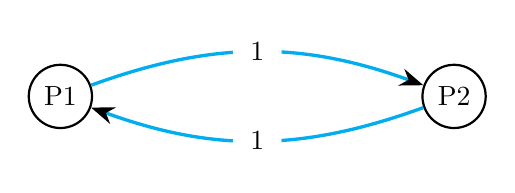
\begin{tikzpicture}
		\begin{scope}[every node/.style={circle,thick,draw}]
			\node (P1) at (0,3) {P1};
			\node (P2) at (5,3) {P2} ;
		\end{scope}
		
		\begin{scope}[>={Stealth[black]},
			every node/.style={fill=white,circle},
			every edge/.style={draw=cyan,very thick}]
			\path [->] (P1) edge[bend left=20] node {$1$} (P2);
			\path [->] (P2) edge[bend left=20] node {$1$} (P1);
		\end{scope}
	\end{tikzpicture}
\end{center}
	
\noindent Suppose the iterative process of equation is run with $\pi^{(0) T}=\left(\begin{array}{ll}0.25 & 0.75\end{array}\right)$. The iterates will not converge no matter how long the process is run. The iterates ${\pi}^{(k) T}$ flip-flop indefinitely between ( $\left.\begin{array}{ll}0.25 & 0.75\end{array}\right)$ when $k$ is even and $\left(\begin{array}{ll}0.75 & 0.25\end{array}\right)$ when $k$ is odd.\\

\begin{thm}[Eigen Values And Eigen Vectors]{thm:eigen}
	For a matrix $\mathbf{A} \in \mathbb{C}^{n \times n}$, the scalars $\lambda$ and the vectors $\mathbf{x}_{n \times 1} \neq \mathbf{0}$ satisfying $\mathbf{A x}=\lambda \mathbf{x}$ are the respective eigenvalues and eigenvectors for $\mathbf{A}$. A row vector $\mathbf{y}^{T}$ is a left-hand eigenvector if $\mathbf{y}^{T} \mathbf{A}=\lambda \mathbf{y}^{T}$.
\end{thm}

\noindent For the above 2-node simple web, it's matrix has eigenvalues 1 \& -1 which are of same magnitude.
\begin{thm}[Spectrum And Spectrum Radius]{thm:spectrum}
	\noindent The set $\sigma(\mathbf{A})$ of distinct eigenvalues is called the spectrum of $\mathbf{A}$, and the spectral radius of $\mathbf{A}$ is the nonnegative number
    $$
	\rho(\mathbf{A})=\max _{\lambda \in \sigma(\mathbf{A})}|\lambda| .
	$$
	\noindent The circle in the complex plane that is centered at the origin and has radius $\rho(\mathbf{A})$ is called the spectral circle
\end{thm}
	
\begin{thm}[Periodic Matrix]{thm:periodicmatrix}
	\noindent A square matrix A such that the matrix power $A^{k+1} = A$ for some positive integer k, is called a periodic matrix. If k is least such integer, then the matrix is said to have period k. For k = 1 A is idempotent.
\end{thm}

\noindent If matrix is not periodic then it is aperiodic(k=0).
Note: k+1 eigen-values lie on the spectral circle.
	
\noindent Periodicity of the transition matrix H is resulting in problem of cycle.\\
\\
\noindent Therefore, the PageRank convergence problems caused by sinks and cycles can be overcome if H is modified slightly so that it is a Markov matrix with these desired properties to get desired output. Further, If our Google matrix some how become aperiodic then we can get PageRank vector just by applying power method with iteration formula regardless of the starting probability vector.

\noindent Now, we know that for any starting probability vector, the power method applied to a Markov matrix M converges to a unique positive vector called the stationary vector as long as P is stochastic, irreducible, and aperiodic.

\subsection{Stochasticity Adjustment}
\noindent Imagine a web surfer who bounces along randomly following the hyperlink structure of the Web. In the long run, the proportion of time the random surfer spends on a given page is a measure of the relative importance of that page. That is, when he arrives at a page with several outlinks, he chooses one at random, hyperlinks to this new page, and continues this random decision process indefinitely. This random surfer encounters some problems. He gets caught whenever he enters a dangling node. And on the Web there are plenty of nodes dangling, e.g., pdf files, image files, data tables, etc.

\noindent The $0^T$ rows of H are replaced with 1/n $e^T$ , thereby making H stochastic. As a result, the random surfer, after entering a dangling node, can now hyperlink to any page at random.\\

\noindent For the tiny 6-node web, Our transition matrix H can be made stochastic matrix called S by simply making RankOne update to H

$$
\mathbf{S}=\left[\begin{array}{cccccc}
	0 & 1 / 3 & 1 / 3 & 1 / 3 & 0 & 0 \\
	1 / 3 & 0 & 1 / 3 & 0 & 0 & 1 / 3 \\
	1/6 & 1/6 & 1/6 & 1/6 & 1/6 & 1/6 \\
	0 & 0 & 0 & 0 & 1 / 2 & 1 / 2 \\
	0 & 0 & 0 & 0 & 0 & 1 \\
	1 / 2 & 0 & 0 & 0 & 1 / 2 & 0
	\end{array}\right]
$$

\noindent For any transition matrix H, stochastic matrix S can be calculated using following formula\\
$$\mathbf{S}=\mathbf{H}+\mathbf{a}\left(1 / n \mathbf{e}^{T}\right)$$
where $\mathbf{e}^{T}$ is row vector with all entries 1\\
\noindent $\mathbf{a}$ is binary column vector called dangling node vector.\\
Entries of $\mathbf{a}$, $a_{i}=1$ if page $i$ is a dangling node and 0 otherwise.
\\
\noindent This adjustment guarantees that $\mathbf{S}$ is stochastic, and thus, is the transition probability matrix for a Markov chain. However, it alone cannot guarantee the convergence results we desired. (That is, that a unique positive $\pi^{T}$ exists) 

\subsection{Primitivity Adjustment}

A primitive matrix is both irreducible and aperiodic. Thus, the PageRank vector of the chain exists, is unique, and can be found by a simple power iteration.\\
\begin{thm}[Positive Matrix]{thm:positivematrix}
	A matrix $P$ is positive if every entry is positive, we write $P>0$ and matrix $P$ is nonnegative if every entry is zero or positive, we write $P \geq 0$.\\
	Primitive Matrix: A square non-negative real matrix $P$ is said to be primitive if there exists a positive integer $k$ such that $P^{k}>0$.
\end{thm}

\noindent The random surfer argument for the primitivity adjustment goes like this. While it is true that surfers follow the hyperlink structure of the Web, at times they get bored and abandon the hyperlink method of surfing by entering a new destination in the browser's URL line. When this happens, the random surfer, like a Star Trek character, "teleports" to the new page, where he begins hyperlink surfing again, until the next teleportation, and so on.\\
\\
To model this mathematically, consider new matrix $\mathbf{G}$, such that
$$
\mathbf{G}=\alpha \mathbf{S}+(1-\alpha) 1 / n \mathbf{e e}^{T},
$$
where $\alpha$ is a scalar between 0 and 1. $\mathrm{G}$ is called the Google matrix. In this model, $\alpha$ is a parameter that controls the proportion of time the random surfer follows the hyperlinks as opposed to teleporting. Suppose $\alpha=0.8$. Then $80 \%$ of the time the random surfer follows the hyperlink structure of the Web and the other $20 \%$ of the time he teleports to a random new page. The teleporting is random because the teleportation matrix $\mathbf{E}=1 / n$ ee $^{T}$ is uniform, meaning the surfer is equally likely, when teleporting, to jump to any page.
\\
\\
There are several consequences of the primitivity adjustment:\\
\\
Matrix G is the convex combination of the two stochastic matrices $\mathbf{S}$ and $\mathbf{E}=1 / n \mathbf{e e}^{T}$ hence it is stochastic.\\
\\
\begin{thm}[Norm]{thm:norm}
	In the applications involving PageRank and Markov chains, it's more natural (and convenient) to use the vector 1 -norm defined by
	$$
	\|\mathbf{x}\|_{1}=\sum_{i=1}^{n}\left|x_{i}\right|
	$$
\end{thm}

\begin{thm}[Perron-Frobenius Theorem]{thm:perronthm}
	If $\mathbf{A}_{n \times n} \geq \mathbf{0}$ is irreducible, then each of the following is true.\\
	1. $r=\rho(\mathbf{A})>0$.\\
	2. $r \in \sigma(\mathbf{A}) \quad(r$ is the Perron root $)$.\\
	3. alg mult $_{\mathbf{A}}(r)=1$. (the Perron root is simple).\\
	4. There exists an eigenvector $\mathbf{x}>\mathbf{0}$ such that $\mathbf{A} \mathbf{x}=r \mathbf{x}$.\\
	5. The Perron vector is the unique vector defined by
	$$
	\mathbf{A p}=r \mathbf{p}, \quad \mathbf{p}>\mathbf{0},\|\mathbf{p}\|_{1}=1,
	$$
	and, except for positive multiples of $\mathbf{p}$, there are no other nonnegative eigenvectors for $\mathbf{A}$, regardless of the eigenvalue.\\
	6. $r$ need not be the only eigenvalue on the spectral circle of $\mathbf{A}$.
\end{thm}

\noindent $\mathrm{G}$ is primitive because $\mathrm{G}^{k}>0$ for some $k$. (In fact, this holds for $k=1 .$ ) G is irreducible as well as aperiodic. G is primitive so irreducibility and aperiodicity are trivially enforced. By Perron-Frobenius Theorem there exists a unique positive probability vector $\pi^{T}$ exists, and it can be obtained by applying power method to $\mathrm{G}$.

\noindent $\mathrm{G}$ is completely dense, which is a very bad thing, computationally. Fortunately, $\mathrm{G}$ can be written as a rank-one update to the very sparse hyperlink matrix $\mathbf{H}$. This is computationally advantageous.
$$
\begin{aligned}
	\mathbf{G} &=\alpha \mathbf{S}+(1-\alpha) 1 / n \mathbf{e e}^{T} \\
	&=\alpha\left(\mathbf{H}+1 / n \mathbf{a e}^{T}\right)+(1-\alpha) 1 / n \mathbf{e e}^{T} \\
	&=\alpha \mathbf{H}+(\alpha \mathbf{a}+(1-\alpha) \mathbf{e}) 1 / n \mathbf{e}^{T} .
\end{aligned}
$$
In summary, Google's adjusted PageRank method is
$$
\boldsymbol{\pi}^{(k+1) T}=\boldsymbol{\pi}^{(k) T} \mathbf{G},
$$
which is simply the power method applied to $\mathrm{G}$.
\section{COMPUTATION OF THE PAGERANK VECTOR}

The PageRank problem can be stated in two ways:\\
\noindent 1. Solve the following eigenvector problem for $\pi^{T}$.
$$
\begin{array}{r}
	\pi^{T}=\pi^{T} \mathrm{G}, \\
	\pi^{T} \mathrm{e}=1 .
\end{array}
$$
\noindent 2. Solve the following linear homogeneous system for $\pi^{T}$.
$$
\begin{aligned}
	\pi^{T}(\mathbf{I}-\mathbf{G}) &=\mathbf{0}^{T} \\
	\pi^{T} \mathbf{e} &=1 .
\end{aligned}
$$

\noindent In the first system, the goal is to find the normalized dominant lefi-hand eigenvector of $\mathrm{G}$ corresponding to the dominant eigenvalue $\lambda_{1}=1 .\left(\mathrm{G}\right.$ is a stochastic matrix, so $\left.\lambda_{1}=1 .\right)$ In the second system, the goal is to find the normalized left-hand null vector of $\mathbf{I}-\mathbf{G}$. Both systems are subject to the normalization equation $\pi^{T} e=1$, which insures that $\pi^{T}$ is a probability vector.
	
\noindent Returning again to 6-node graph, for $\alpha=0.9$,
	
$$
\begin{aligned}
	\mathbf{G}=0.9 \mathbf{H}+\left(0.9\left(\begin{array}{l}
		0 \\
		1 \\
		0 \\
		0 \\
		0 \\
		0
\end{array}\right)+0.1\left(\begin{array}{l}
		1 \\
		1 \\
		1 \\
		1 \\
		1 \\
		1
\end{array}\right)\right) 1 / 6\left(\begin{array}{llllll}
		1 & 1 & 1 & 1 & 1
		\end{array}\right) \\
		=\left(\begin{array}{cccccc}
		1 / 60 & 19 / 60 & 19 / 60 & 19 / 60 & 1 / 60 & 1 / 60 \\
		19 / 60 & 1 / 60 & 19 / 60 & 1 / 60 & 1 / 60 & 19 / 60 \\
		1 / 6 & 1 / 6 & 1 / 6 & 1 / 6 & 1 / 6 & 1 / 6 \\
		1 / 60 & 1 / 60 & 1 / 60 & 1 / 60 & 7 / 15 & 7 / 15 \\
		1 / 60 & 1 / 60 & 1 / 60 & 7 / 15 & 1 / 60 & 11 / 15 \\
		7 / 15 & 1 / 60 & 1 / 60 & 1 / 60 & 7 / 15 & 1 / 60
    \end{array}\right) .
\end{aligned}
$$


\noindent Google's PageRank vector is the stationary vector of $\mathrm{G}$ and is given by
$$
\pi^{T}=\left(\begin{array}{cccccc}
	P_1 & P_2 & P_3 & P_4 & P_5 & P_6 \\
	0.1939 & 0.09295 & 0.1208 & 0.09295 & 0.2078 & 0.2915
\end{array}\right) .
$$

\noindent The interpretation of $\pi_{1}=0.1939$ is that $19.39 \%$ of the time the random surfer visits $P_1$. Therefore, the pages in tiny 6-node web can be ranked by their importance as ($\begin{matrix}
3 & 5 & 4 & 5 & 2 & 1
\end{matrix}$), meaning $P_6$ is the most important page and $P_2$ \& $P_4$ are the least important page, according to the PageRank definition of importance.\\


\noindent However, for a web-sized matrix like Google's, solving eigenvalue-eigenvector problem is not possible.  For Google,
n = 8.1 billion, so one can understand their gigantic size when it comes to storage.
%	Other iterative methods, such as GMRES or BICGSTAB, while faster, require the storage
%	of multiple vectors. 
The power method is one of the oldest and simplest iterative methods for finding the dominant eigenvalue and eigenvector of a matrix. However, the power method is known for its tortoise-like speed.

\noindent There are several good reasons for their choice.

\noindent Modifying and storing elements of the Google matrix is not feasible. %Even though H is very sparse, its enormous size and lack of structure preclude the use of direct methods. 
Instead, matrix-free methods, such as the class of iterative methods, are preferred. First, the power method is simple. The implementation and programming are elementary. In addition, the power method applied to $\mathrm{G}$  can actually be expressed in terms of the very sparse $\mathbf{H}$.
$$
\begin{aligned}
	\boldsymbol{\pi}^{(k+1) T} &=\boldsymbol{\pi}^{(k) T} \mathbf{G} \\
	&=\alpha \boldsymbol{\pi}^{(k) T} \mathbf{S}+\frac{1-\alpha}{n} \boldsymbol{\pi}^{(k) T} \mathbf{e} \mathbf{e}^{T} \\
	&=\alpha \boldsymbol{\pi}^{(k) T} \mathbf{H}+\left(\alpha \boldsymbol{\pi}^{(k) T} \mathbf{a}+1-\alpha\right) \mathbf{e}^{T} / n .
	\end{aligned}
$$
	
\noindent The vector-matrix multiplications $\left(\boldsymbol{\pi}^{(k) T} \mathbf{H}\right)$ are executed on the extremely sparse $\mathbf{H}$, and $\mathbf{S}$ and $\mathbf{G}$ are never formed or stored, only their rank-one components, a and $\mathbf{e}$, are needed.\\
	
\begin{thm}[]{}
	Given probability vector $\pi^{(0)T}>0$ and stochastic matrix G then $\pi^{(k)T}>0$ is also probability vector for all positive integers.
\end{thm}
	
\noindent We know till now that the sequence of PageRank Vector $(\boldsymbol{\pi}^{(k)})$ is convergent and each term of the sequence is probability vector.
	
\noindent For page ranking precision up to 3-4 decimal places is enough as PageRank is finally combined with the content and popularity index. Now, how many iteration do we need to get desired precision?
	
\begin{thm}[Generalized Google Matrix]{thm:googlematrix}
	We defined the Google matrix as $\mathbf{G}=\alpha \mathbf{S}+(1-\alpha) 1 / n \mathbf{e e}^{T}$. However, we broaden this to include a more general Google matrix, where the fudge factor matrix $\mathbf{E}$ changes from the uniform matrix $\frac{1}{n} \mathbf{e e}^{T}$ to $\mathbf{e v}^{T}$, where $\mathbf{v}^{T}>\mathbf{0}$ is a probability vector.
\end{thm}
	
\noindent The answer comes from the theory of Markov chains. In general, the asymptotic rate of convergence of the power method applied to a matrix depends on the ratio of the two eigenvalues that are largest in magnitude, denoted $\lambda_{1}$ and $\lambda_{2}$. 

\begin{thm}[]{}
If the spectrum of the stochastic matrix $\mathbf{S}$ is $\left\{1, \lambda_{2}, \lambda_{3}, \ldots, \lambda_{n}\right\}$, then the spectrum of the Google matrix $\mathbf{G}=\alpha \mathbf{S}+(1-\alpha) \mathbf{e v}^{T}$ is $\left\{1, \alpha \lambda_{2}, \alpha \lambda_{3}, \ldots, \alpha \lambda_{n}\right\}$, where $\mathbf{v}^{T}$ is a probability vector.
\end{thm}
	
\noindent Precisely, the asymptotic convergence rate is the rate at which $\left|\lambda_{2} / \lambda_{1}\right|^{k} \rightarrow 0$. For stochastic matrices such as $\mathbf{G}, \lambda_{1}=1$, so $\left|\lambda_{2}\right|$ governs the convergence. Since $\mathbf{G}$ is also primitive, $\left|\lambda_{2}\right|<1$. In general, numerically finding $\lambda_{2}$ for a matrix requires computational effort that one is not willing to spend just to get an estimate of the asymptotic rate of convergence.\\
	
\begin{thm}[Subdominant Eigen Value]{thm:subdominanteigen}
	Norm of subdominant Eigenvalue of the Google Matrix
	For the Google matrix $\mathbf{G}=\alpha \mathbf{S}+(1-\alpha) 1 / n \mathbf{e e}^{T}$,
	$$
	\alpha||\lambda_{2}|| \leq \alpha .
	$$
	\\
Therefore, the asymptotic rate of convergence of the PageRank power method of equation is the rate at which $(\alpha||\lambda_{2}||)^{k} \rightarrow 0$.
\end{thm}
	
\noindent Furthermore, the link structure of the Web makes it very likely that $\left|\lambda_{2}(\mathbf{G})\right| \approx \alpha$. As a result, convergence of PageRank vector depend upon parameter $\alpha$. Google founders Brin and Page use $\alpha=.85$, and at last report, this is still the value used by Google. $\alpha^{50}=.85^{50} \approx .000296$, which implies that at the 50th iteration one can expect roughly 3-4 places of accuracy in the approximate PageRank vector. This degree of accuracy is apparently adequate for Google's ranking needs. Mathematically, ten places of accuracy may he needed to distinguish between elements of the PageRank vector, but when PageRank scores are combined with content and popularity score, high accuracy may be less important. Thus, now we are able to calculate PageRank for any graph weather it is of order 10s or 1Billions.\\
\\
\noindent Google's PageRank algorithm is in use from early 90s, so as time goes, most likely traditional method going to fade forcing mathematicians to work on newer methods for calculating PageRank.
\end{document}